\section{3D-Daten}
\label{app:3D}
\subsection{Platine}
Die Platine wurde zur Validierung des Designs als 3D-Modell dargestellt.
\begin{figure}[h] 
	\centering
	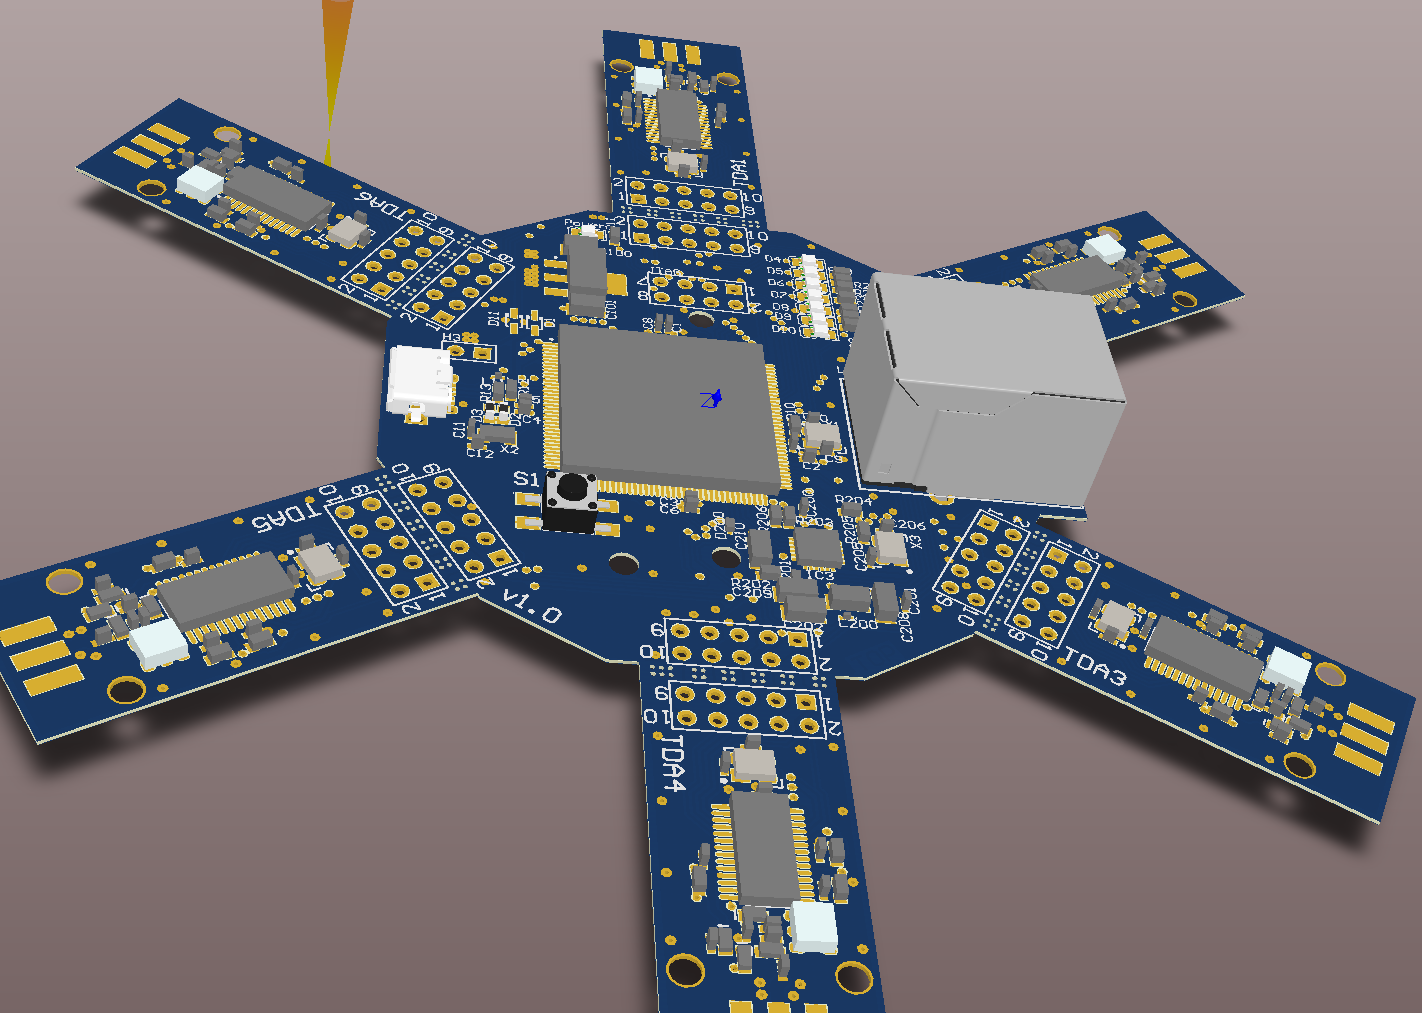
\includegraphics[width=\textwidth]{Abbildungen/Aufnahmen/Bilder/Altium/3D2}
	\caption{3D-Modell der Basisstation in Altium Designer}
	\label{fig:3D}
\end{figure}
\subsection{Gehäuse}
\label{app:Gehäuse}
Mit der Software SolidWorks wurde ein Gehäuse für die Platine erstellt.
\begin{figure}[h]
\centering
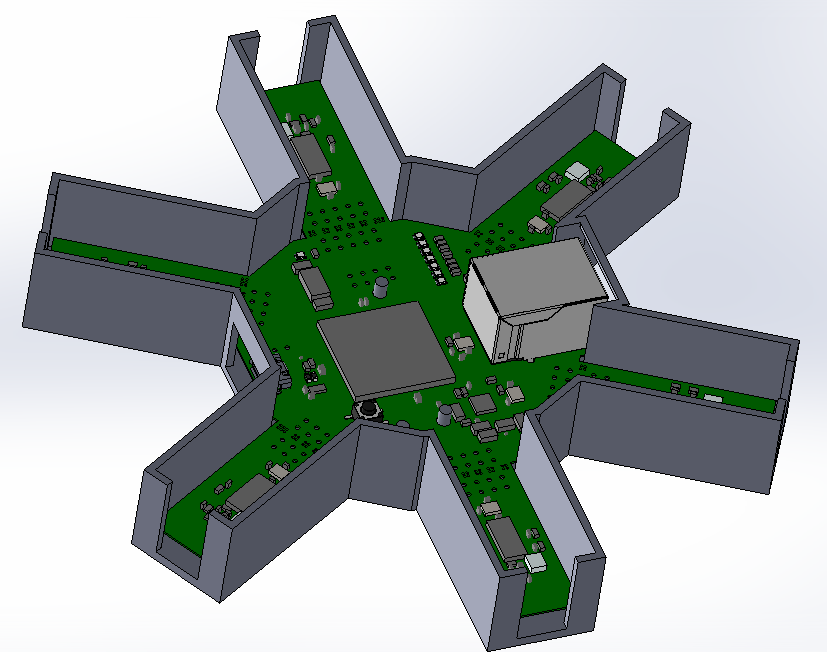
\includegraphics[width=\linewidth]{Abbildungen/Aufnahmen/Bilder/SolidWorks/BoxBildschirmSW}
\caption{Erstellte Box zum Schutz der Basisstation in der Software SolidWorks}
\label{fig:boxbildschirmsw}
\end{figure}




